\documentclass[journal]{vgtc}                % final (journal style)
%\documentclass[review,journal]{vgtc}         % review (journal style)
%\documentclass[widereview]{vgtc}             % wide-spaced review
%\documentclass[preprint,journal]{vgtc}       % preprint (journal style)

%% Uncomment one of the lines above depending on where your paper is
%% in the conference process. ``review'' and ``widereview'' are for review
%% submission, ``preprint'' is for pre-publication, and the final version
%% doesn't use a specific qualifier.

%% Please use one of the ``review'' options in combination with the
%% assigned online id (see below) ONLY if your paper uses a double blind
%% review process. Some conferences, like IEEE Vis and InfoVis, have NOT
%% in the past.

%% Please note that the use of figures other than the optional teaser is not permitted on the first page
%% of the journal version.  Figures should begin on the second page and be
%% in CMYK or Grey scale format, otherwise, colour shifting may occur
%% during the printing process.  Papers submitted with figures other than the optional teaser on the
%% first page will be refused. Also, the teaser figure should only have the
%% width of the abstract as the template enforces it.

%% These few lines make a distinction between latex and pdflatex calls and they
%% bring in essential packages for graphics and font handling.
%% Note that due to the \DeclareGraphicsExtensions{} call it is no longer necessary
%% to provide the the path and extension of a graphics file:
%% 
\includegraphics{diamondrule} is completely sufficient.
%%
\ifpdf%                                % if we use pdflatex
  \pdfoutput=1\relax                   % create PDFs from pdfLaTeX
  \pdfcompresslevel=9                  % PDF Compression
  \pdfoptionpdfminorversion=7          % create PDF 1.7
  \ExecuteOptions{pdftex}
  \usepackage{graphicx}                % allow us to embed graphics files
  \DeclareGraphicsExtensions{.pdf,.png,.jpg,.jpeg} % for pdflatex we expect .pdf, .png, or .jpg files
\else%                                 % else we use pure latex
  \ExecuteOptions{dvips}
  \usepackage{graphicx}                % allow us to embed graphics files
  \DeclareGraphicsExtensions{.eps}     % for pure latex we expect eps files
\fi%

%% it is recommended to use ``\autoref{sec:bla}'' instead of ``Fig.~\ref{sec:bla}''
\graphicspath{{figures/}{pictures/}{images/}{./}} % where to search for the images

\usepackage{microtype}                 % use micro-typography (slightly more compact, better to read)
\PassOptionsToPackage{warn}{textcomp}  % to address font issues with \textrightarrow
\usepackage{textcomp}                  % use better special symbols
\usepackage{mathptmx}                  % use matching math font
\usepackage{times}                     % we use Times as the main font
\renewcommand*\ttdefault{txtt}         % a nicer typewriter font
\usepackage{cite}                      % needed to automatically sort the references
\usepackage{tabu}                      % only used for the table example
\usepackage{booktabs}                  % only used for the table example
%% We encourage the use of mathptmx for consistent usage of times font
%% throughout the proceedings. However, if you encounter conflicts
%% with other math-related packages, you may want to disable it.

%% In preprint mode you may define your own headline.
%\preprinttext{To appear in IEEE Transactions on Visualization and Computer Graphics.}

%% If you are submitting a paper to a conference for review with a double
%% blind reviewing process, please replace the value ``0'' below with your
%% OnlineID. Otherwise, you may safely leave it at ``0''.
\onlineid{0}

%% declare the category of your paper, only shown in review mode
\vgtccategory{Research}
%% please declare the paper type of your paper to help reviewers, only shown in review mode
%% choices:
%% * algorithm/technique
%% * application/design study
%% * evaluation
%% * system
%% * theory/model
\vgtcpapertype{application/design study}

%% Paper title.
\title{How climate change affects bird migration}

%% This is how authors are specified in the journal style

%% indicate IEEE Member or Student Member in form indicated below
\author{Gabriela Slavova, Henrique Dias, Nimo Beeren}
\authorfooter{
%% insert punctuation at end of each item
\item
Gabriela Slavova, Henrique Dias and Nimo Beeren are with Eindhoven University of
Technology. E-mail: \{g.slavova, h.a.coelho.dias, n.beeren\}@student.tue.nl.
}

%other entries to be set up for journal
%\shortauthortitle{Biv \MakeLowercase{\textit{et al.}}: Global Illumination for Fun and Profit}
%\shortauthortitle{Firstauthor \MakeLowercase{\textit{et al.}}: Paper Title}

%% Abstract section.
\abstract{Abstract text%
} % end of abstract

%% Keywords that describe your work. Will show as 'Index Terms' in journal
%% please capitalize first letter and insert punctuation after last keyword
\keywords{Climate change, bird migration.}

%% ACM Computing Classification System (CCS). 
%% See <http://www.acm.org/class/1998/> for details.
%% The ``\CCScat'' command takes four arguments.

%\CCScatlist{ % not used in journal version
% \CCScat{K.6.1}{Management of Computing and Information Systems}%
%{Project and People Management}{Life Cycle};
% \CCScat{K.7.m}{The Computing Profession}{Miscellaneous}{Ethics}
%}

%% Uncomment below to include a teaser figure.
%\teaser{
%  \centering
%  \includegraphics[width=\linewidth]{CypressView}
%  \caption{In the Clouds: Vancouver from Cypress Mountain. Note that the teaser may not be wider than the abstract block.}
%	\label{fig:teaser}
%}

%% Uncomment below to disable the manuscript note
%\renewcommand{\manuscriptnotetxt}{}

%% Copyright space is enabled by default as required by guidelines.
%% It is disabled by the 'review' option or via the following command:
% \nocopyrightspace

\vgtcinsertpkg

%%%%%%%%%%%%%%%%%%%%%%%%%%%%%%%%%%%%%%%%%%%%%%%%%%%%%%%%%%%%%%%%
%%%%%%%%%%%%%%%%%%%%%% START OF THE PAPER %%%%%%%%%%%%%%%%%%%%%%
%%%%%%%%%%%%%%%%%%%%%%%%%%%%%%%%%%%%%%%%%%%%%%%%%%%%%%%%%%%%%%%%

\begin{document}

%% The ``\maketitle'' command must be the first command after the
%% ``\begin{document}'' command. It prepares and prints the title block.

%% the only exception to this rule is the \firstsection command
\firstsection{Introduction}

\maketitle

In recent times, it has become increasingly clear to most people that climate change is affecting life on Earth. As temperatures rise globally, many animals are forced to adapt to their environment \cite{parmesan2007pheno,gaughan2009domestic,root2003fingerprints}. Among the best-documented instances of such adaptation are changes in bird migration times \cite{miller2008bird,visser2008climate,jenni2003timing}. This paper presents an interactive visualization with the goal to communicate these findings.

\subsection{Problem Description}

Despite evidence presented in numerous studies \cite{solomon2007climate,parry2007climate}, it has proved to be difficult to communicate the effects of climate change to people \cite{lee2015predictors,brulle2012shifting,moser2011communicating}. We believe that visualizing effects that can be observed in everyday life is an important way of fostering public engagement. One such effect is the change in the time of the year during which migratory birds can be observed in their breeding habitat. As global temperatures increased, birds have been migrating to their breeding habitats earlier in the year \cite{cotton2003avian,huppop2003north,marra2005influence}. Using a visual approach, we intend to show this correlation in a way that is interpretable to experts and non-experts alike.

Both bird migration and surface temperature changes are cyclic processes with an annual period. In order to infer trends in these processes, we should consider data from multiple years, or even decades. However, because of the cyclic nature, it is difficult to directly compare one year to another. One of the challenges of this problem is to visualize trends over the long term, without obscuring the patterns that occur every year.

Another attribute that these processes have in common is that they are both geographic. That is, both produce data that is associated with a particular place on Earth \cite{iso2014geo}. It is essential to visualize both in such a way that one does not obscure the other, while their correlation is still visible.

\section{Data Analysis}

\subsection{Domain Data Specification}

In order to visualize the problem, we need two different datasets: one that includes information about birds migration and one including temperature changes over the years.

For the first needed dataset we have chosen the eBird Basic Dataset \cite{ebird2020data}. The eBird citizen science project is unmatched in scale, containing over 600 million observations, including nearly every bird species on Earth \cite{strimas2020ebird}. Submissions are individually reviewed to ensure accuracy of information. As people are contributing to this dataset continuously, the information inside is up-to-date, but the record also goes many years back.

For the second, we have chosen the GISTEMP dataset \cite{gistemp} by NASA, which provides the temperature data from 1880 up to 2020 in a regular 2° by 2° grid. The main advantage of this dataset compared to other temperature datasets we found is that this one uses the temperature anomalies. These anomalies are relative to a 30-year period between 1951 and 1980. By using anomalies instead of absolute values \cite{gistempanomalies}, it is easier to see how much colder or warmer a certain place is. 

\subsection{Data Abstraction: What}
\label{subsec:data-abs-what}

The eBird Basic Dataset \cite{ebird2020data} consists of a large static table containing items that each correspond to a particular observation of a bird or a group of birds. For each observation, a number of attributes are provided, though we are only interested in the following subset:

\paragraph{Species} A categorical attribute represented by the scientific name, e.g. \textit{Anas platyrhynchos}. The eBird taxonomy\cite{ebird2019taxonomy} specifies exactly what is meant with these names.

\paragraph{Date} An ordered, quantitative and diverging attribute in year-month-day format (yyyy-mm-dd).

\paragraph{Location} A spatial attribute consisting of a vector with components latitude and longitude. Each component is itself an ordered, quantitive and cyclic attribute represented as decimal degrees, where positive values denote N/W and negative values denote S/E for latitude/longitude respectively. The precision varies between observations, but is typically 0.001 degrees or more precise (which is less than 1 km on Earth's surface).

\paragraph{Count} An ordered, quantitative and diverging attribute represented as an integer. Since participants are allowed to group multiple birds in a single observation, the value can be 1 or greater.

\vspace{2mm}

We perform a number of transformations on the original dataset for the purpose of our visualization. First, we limit ourselves to a single species, since different species exhibit significantly different migratory behavior. We chose the Barn Swallow (\textit{Hirundo rustica}) because it is a relatively common migratory bird, and it typically migrates over a large distance \cite{turner1989swallow}. Next, we restrict the dataset geographically to Europe and Africa. These transformations allow us to focus on a general population of birds. Finally, we exclude observations outside the years 1950-2020, since that matches the domain of the temperature dataset we use.

\vspace{2mm}

The GISTEMP dataset \cite{gistemp} consists of a large static multidimensional scalar field, whose dimensions are the latitude, the longitude and the date. For each point in space-time, a temperature anomaly value is available. The description of each dimension and the value:

\paragraph{Latitude} An ordered quantitative cyclic attribute represented as decimal degrees, varying from -90.0 to 90.0.

\paragraph{Longitude} An ordered quantitative cyclic attribute represented as decimal degrees, varying from -180.0 to 180.0.

\paragraph{Temperature Anomaly} A quantitive attribute represented in degrees Celcius.

\paragraph{Date} An ordered, quantitive and diverging attribute in year-month format (yyyy-month).

\section{Task Analysis}
\label{tasks}

\subsection{Domain Specific Tasks}

This visualization is designed to be used by a large variety of specialists and non-specialists alike. An ornithologist could study the migration of the Barn Swallow using the provided visualization. It is also suitable for the needs of climate  change activists who wants to prove a point about a real prolem or a curious person without specific domain knowledge who wants to see the effects of climate change on the nature. The tasks that  these people could undertake are described below.

\paragraph{Task 1: Analyze correlation between temperature change and the timing of bird migration} One of the observations that can be achieved with this visualization is showing the migration of birds in relation to the change in temperature over time. This can be done by choosing a bird species and comparing timing of their migration with respect to the temperatures for the specific time and the same migration in a different time span before or after the chosen one.  The question that would be answered by this task is: how are temperature and the timing of bird migration correlated?

\paragraph{Task 2: Characterize the migration behavior of a species} Another thing that is possible to be visualized is the migration pattern of a specific type of bird over the course of a year. This can be done be choosing a bird species and following its migration behavior through a chosen year. The question that would be answered by this task is: what is the general migration behavior pattern for a particular bird species?

\paragraph{Task 3: Identify species that respond most to temperature change} Different types of birds respond differently to a change in temperature. The tool can help visualize which types of birds are affected by the rising temperatures more than others. This can be done by comparing the migration behavior in relation to the temperature over time, for a set of species. The question that would be answered by this task is: which bird species respond to temperature change the most?

\subsection{Task Abstraction: Why}

\paragraph{Task 1: Analyze correlation between temperature change and the timing of bird migration} The high-level analyze action that this task performs is consume and more precisely discover. This is because discover is related to the act of verifying or disproving of a hypothesis which is exactly the intention behind this task. The mid-level search action is explore as the user doesn't know the location of the target or what the target itself is. The low-level query action is compare as the user will compare different data. The target of this task is a correlation.

\paragraph{Task 2: Characterize the migration behavior of a species} The high-level analyze action in this task is discover, because discover is also generally related to the act of observing without knowing specifically the end result. The mid-level search action is explore as the location of the target and the target itself are unknown. The low-level query action is summarize because this task aims to return general overview of the patterns in the data. The target of this task is also a trend.

\paragraph{Task 3: Identify species that respond most to temperature change} The high-level analyze action performed in this task is also discover. The mid-level search action is explore. The low-level query action is identify. The target of this task is outliers.

\section{Visualization and Interaction Design: How}

% Describe and motivate your choices for the visual encodings and interaction design (\emph{How}). You should not think about implementation yet, but rather what visual encodings fit best to address the task/data results presented earlier. You must justify your choices based on the design principles described in the course. Here is where you explicitly link your tasks, questions and data to the design, and argue why the chosen design will enable users to perform the tasks and answer their questions. Explain the main interactions provided in your solution.

\section{Realization}

All of the idealized visualizations were implemented. With that being said, we implemented the temperature anomaly map, the bird frequency map, as well as a line chart showing the average temperature anomaly and bird latitude.

We implemented a web application. Thus, the main technologies in use are HTML, CSS and JavaScript. To manage the application state, we decided to use Svetle\cite{svetle}, a relatively young framework designed to build web apps easily. Despite the existence of more mature frameworks, such as React, Vue.js and Angular, we decided to use Svetle as it is simple to use and enables us to do the implemetation in a short amount of time leaving more time for designing the application.

\begin{figure}[h]
  \centering
  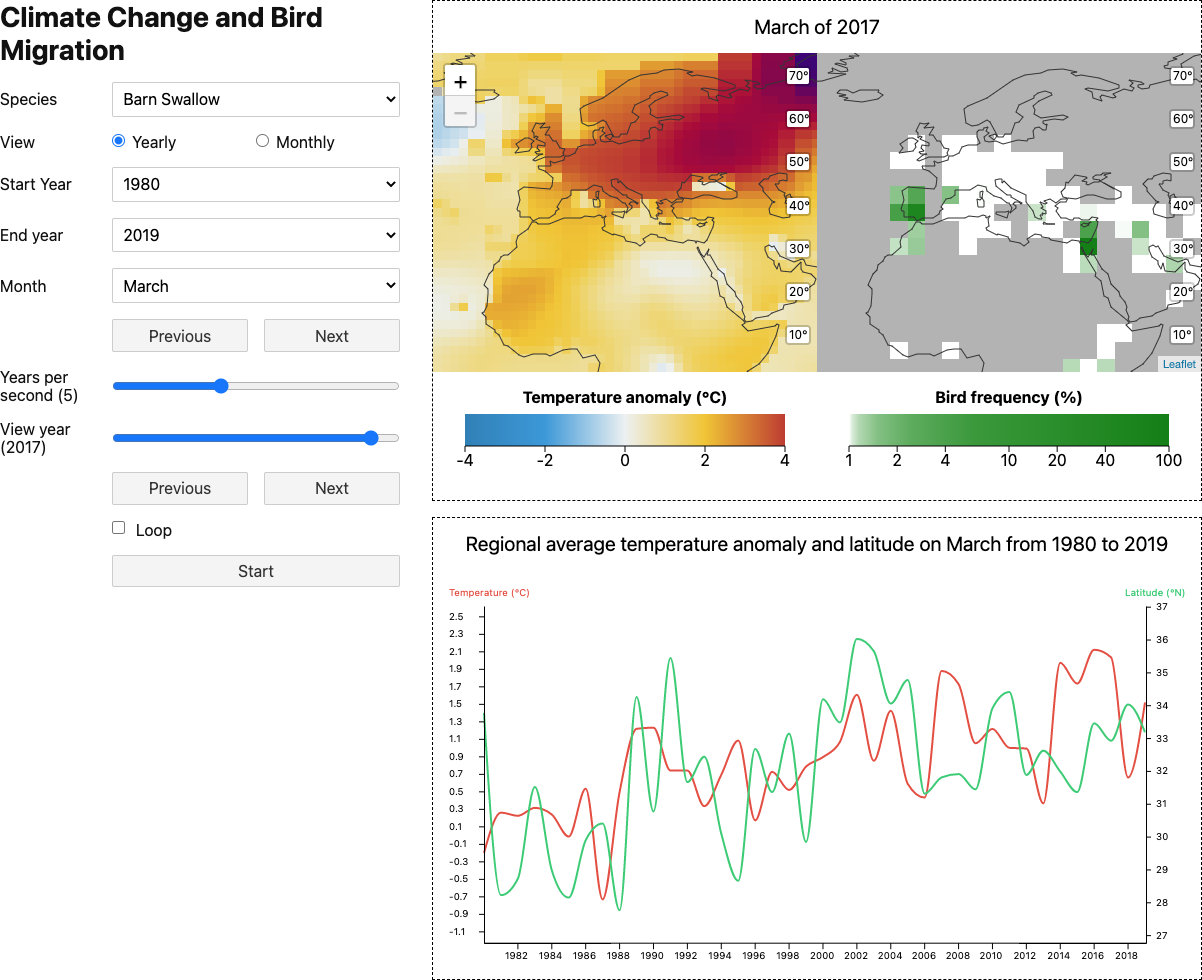
\includegraphics[width=85mm]{app-example.png}
  \caption{``Climate Change and Bird Migration" visualization application overview.}
  \label{fig:app-example}
\end{figure}

\subsection{Controls}

The main point of interaction of the user with the application is the controls. The controls section is a set of dropdown menus, buttons and other types of input. These allow the user to change between different species and view types. According to the selected view type, different options become available.

For the yearly view, the user can select the start and end years, the month, as well as the number of years per second - also known as the speed of the animation. These options affect: (1) the animation over the years, which can be started by pressing ``Start"; and (2) the base data used in the visualization. In addition, while the animation is stopped, the user can choose a specific year to show in the maps.

For the monthly view, the user can choose the month, the number of months per second and the year to view. Similarly to what happens with the yearly view, these options will affect the map animation, as well as the data used in the graph.

Disregarding both views, there is also an option to choose to infinitely repeat the animation by checking the box ``Loop".

\subsection{Maps}

The implementation of the maps resorts to Leaflet \cite{leaflet}, an open-source JavaScript library for interactive maps. With this library, we were able to show two maps side by side, which can be zoomed in and panned. In addition, we also show the latitude on the right side of the maps.

By hovering the cursor over a certain point in the temperature anomalies map, the user is able to see the precise temperature anomaly in that point. The same applies for the bird frequency map.

Both maps are synchronized such that they always show the same area at the same time. Thus, if the user zooms in/out or moves one map, the other one is zoomed in automatically.

Below each map, there is also a scale. This scale, as well as the mapping between a numeric value and a color in the map, were partially implemented by the library D3 \cite{d3js}.

An example of the mentioned features can be seen in Figure \ref{fig:map-example}.

\begin{figure}[h]
  \centering
  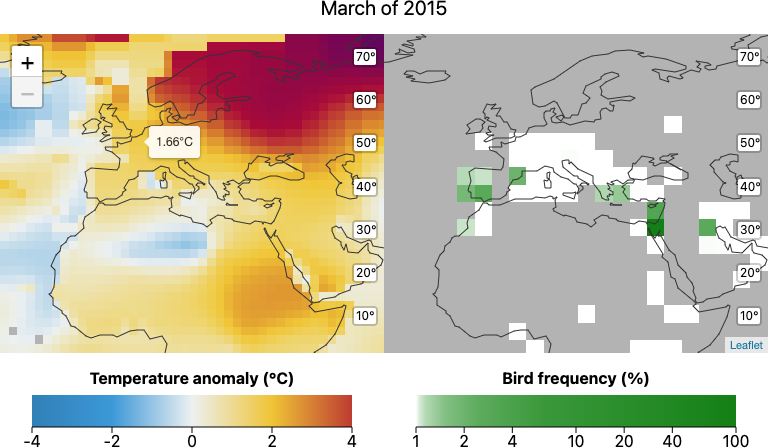
\includegraphics[width=85mm]{map-example}
  \caption{Map example for March 2015, showcasing the latitudes, scales and tooltip functionality.}
  \label{fig:map-example}
\end{figure}

\subsection{Line Chart}

The line chart implemention mainly relies on D3 \cite{d3js}, a JavaScript library that allows for data manipulation and its visualization using Scalable Vector Graphics images (SVGs). The graph can show two views: either month by month, or year by year. The visualization depends on the choosen options. You can see an example of a monthly graph on Figure \ref{fig:montly-graph16} and a yearly graph on \ref{fig:march86-16-graph}.

In addition, the graph view is regional, meaning that the data on the graph is intrisincally related to the map view. The graph only shows the data from the visible area of the map. Thus, if the user zooms in or out in the map, the graph will change to show the information regarding a different map area.

\subsection{Data Processing}

During the development of the application, we had to apply some transformations to the initial data as mentioned in subsection \ref{subsec:data-abs-what}. To do so, we used the programming languages Python and R, as they are both languages tailored for data processing and analytics.

\section{Use Cases}

In this section, we demonstrate how the application can be used to perform the tasks and answer the questions described in Section \ref{tasks}.

\paragraph{How are temperature changes and the timing of bird migration correlated?}

One of the main goals of the application is to analyze possible correlations between the temperature changes and the timing of bird migration. To do so, it is recommended to use the yearly view. The user can select a specific bird species to visualize. However, the default one - Barn Swallow - provides the most clear correlation.

An important choice the user has to make is to pick which month they want to visualize. Some of the months of the year are better to showcase the movement of birds because their migration depends on certain weather conditions and other natural factors. For instance, March is associated with the migrations of most birds to the northern hemisphere.

After choosing a specific month, the user can navigate through the years. This allows the user to compare how the bird movement has changed over the span of several years, while being able to see the changes in temperatures for the same span of time. An example visualization can be seen on Fig. \ref{fig:swallow-map-86} and Fig. \ref{fig:swallow-map-16}.

\begin{figure}[h]
  \centering
  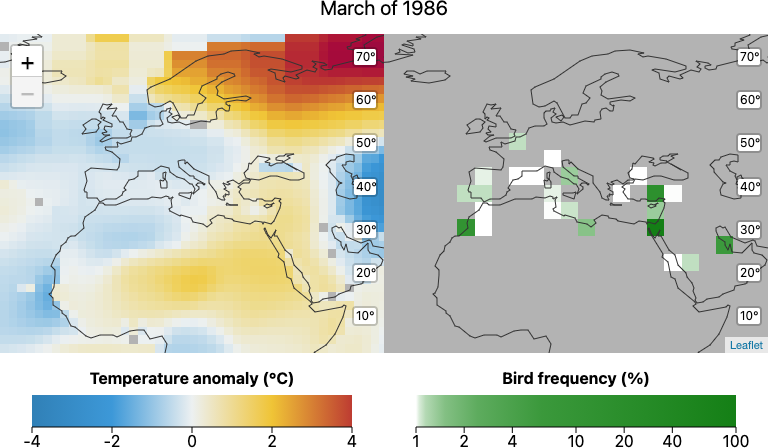
\includegraphics[width=85mm]{march86-map-barnswallow}
  \caption{Maps of temperature anomaly and Barn Swallow latitude position for March 1986.}
  \label{fig:swallow-map-86}
\end{figure}

\begin{figure}[h]
  \centering
  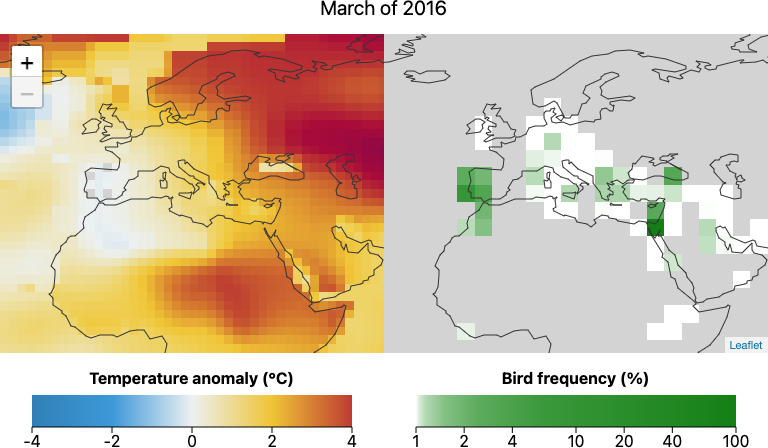
\includegraphics[width=85mm]{march16-map-barnswallow}
  \caption{Maps of temperature anomaly and Barn Swallow latitude position for March 2016.}
  \label{fig:swallow-map-16}
\end{figure}

Instead of manually navigating through the years, a user can select a month, a start and an end year, and press the ``Start" button. This will start an animation showing the chosen month for each year between the start and the end year, inclusively. The speed of the animation can also be customized. There is also a choice of looping the animation, so the user can watch it continuously and spot even the smallest differences.

In some cases the map does not showcase clearly enough the correlation the user is looking for. For these cases there is a line chart that shows the changes of the temperature anomaly and the overall position of the birds on the latitude for a given month and year. The specifications of the graph can be changed by choosing a start year, end year and month. Figure \ref{fig:march86-16-graph} shows an example for a line chart generated for the month of March between the years 1986 and 2016.

\begin{figure}[h]
  \centering
  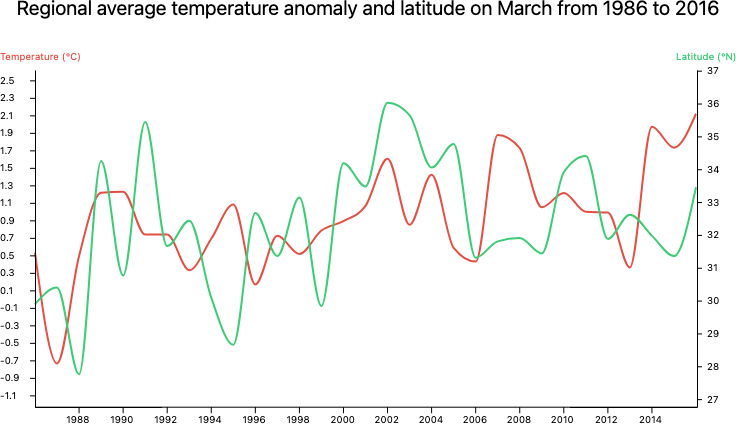
\includegraphics[width=85mm]{march86-16-graph-barnswallow}
  \caption{Line graph showing the variation of the temperature anomalies and Barn Swallow's latitude position for March 1986 to 2016.}
  \label{fig:march86-16-graph}
\end{figure}

\paragraph{What is the general migration behavior pattern for a particular bird species?}

Typically, the migration of birds has a repeated pattern of annual cycles. In order for a user to observe the general migration behavior of a bird species, they have to follow its movement over the course of a year and note the overall pattern. In this case, the monthly view is the most convenient choice. With it, a user can choose the specific bird species that they are interested in, as well as choosing a specific year. Then, by pressing ``Start", the user can visualize an animation, from January to December in the selected year, that shows the position changes over the year. Similarly to the yearly view, there is also an option to change the speed and to infinitely repeat the animation until the user decides to stop.

In conjunction to the map view, there is a line chart showing the general latitude position of the species for each month of the selected year. The line graph can be used to easily spot patterns in different parts of the annual migration cycle. Figure \ref{fig:montly-graph16} shows a monthly line graph for the year of 2016 for the Barn Swallow.

\begin{figure}[h]
  \centering
  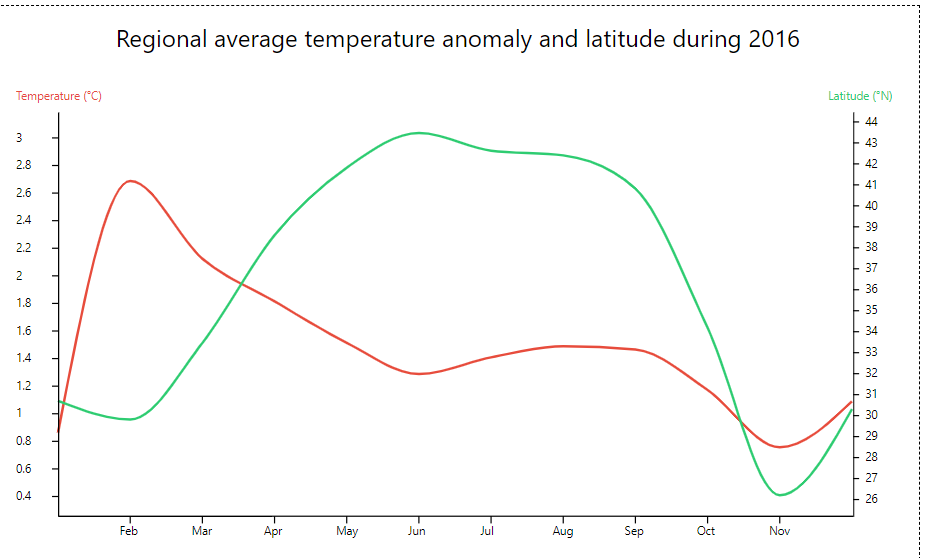
\includegraphics[width=85mm]{montly-graph16-barnswallow}
    \caption{Line graph showing the variation of the temperature anomalies and Barn Swallow's latitude position in 2016.}
  \label{fig:montly-graph16}
\end{figure}

\paragraph{Which bird species respond to temperature change the most?}

To compare the response to temperature changes of different bird species, we recommend the yearly view. Firstly, the user should choose the parameters of interest such as year(s), month and bird species. Then, the user should observe each species, one by one. At any time, the user can change to a different bird species, thus allowing to view the different species' behavior. This is applicable to both the maps and the line chart. For example we can use Figure \ref{fig:swallow-map-16} and Figure \ref{fig:march16-map-blackbird} to compare the behavior of the Barn Swallow and the Eurasian Blackbird during March 2016.

\begin{figure}[h]
  \centering
  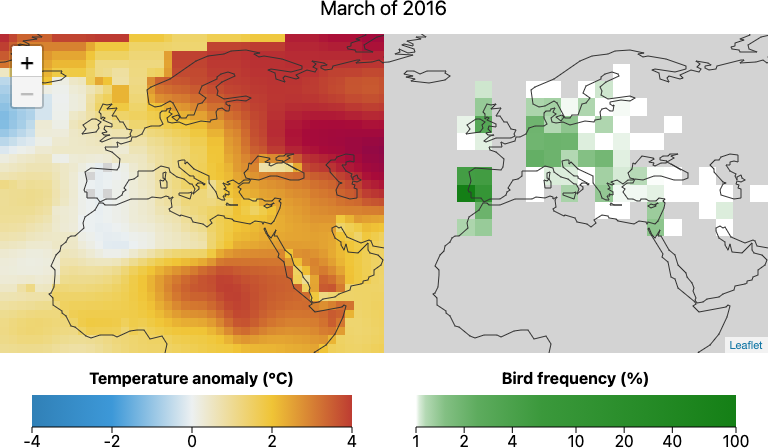
\includegraphics[width=85mm]{march16-map-blackbird}
  \caption{Visualization of maps of temperature anomaly and Eurasian Blackbird latitude porsition for March 2016.}
  \label{fig:march16-map-blackbird}
\end{figure}

\section{Discussion and Conclusion}

% Finally, you will reflect on what you have achieved. For instance, this section should discuss whether you managed to do what you initially planned, whether your initial choices worked well or not, things that you discovered that were not correct, etc. Conclusions about your whole work would be provided.

\bibliographystyle{abbrv}
\bibliography{main}
\end{document}
